%!TEX root = ../dissertation.tex
\chapter{Publications using Orthograph}
\label{papers-using-orthograph}

\addtocounter{section}{1}
\addcontentsline{toc}{section}{A.\arabic{section}\quad Bias in big-data phylogenetics: anchored phylogenomics unravels the evolution of spider flies (Acroceridae) and reveals discordance between nucleotides and amino acids \citep{Gillung2018}}
\citet{Gillung2018}, submitted to MBE
%\includepdf[pages=-]{file} % range without endpoints: from first to last

\addtocounter{section}{1}
\addcontentsline{toc}{section}{A.\arabic{section}\quad Phylogenomics and the evolution of hemipteroid insects \citep{Johnson2018}}
\citet{Johnson2018}, submitted to PNAS
%\includepdf[pages=-]{file} % range without endpoints: from first to last

\includepdf[addtotoc={1,section,1,Evolutionary history of the Hymenoptera \citep{Peters2017},app:Peters2017},pages=-]{appendix/A/Peters2017} % range without endpoints: from first to last

\includepdf[addtotoc={1,section,1,Phylogenetic origin and diversification
of RNAi pathway genes in insects \citep{Dowling2017},app:Dowling2017},pages=-]{appendix/A/Dowling2017}

\includepdf[addtotoc={1,section,1,New insights into the phylogeny of vespid
wasps (Hymenoptera: Aculeata: Vespidae) \citep{Bank2017},app:Bank2017},pages=-]{appendix/A/Bank2017}

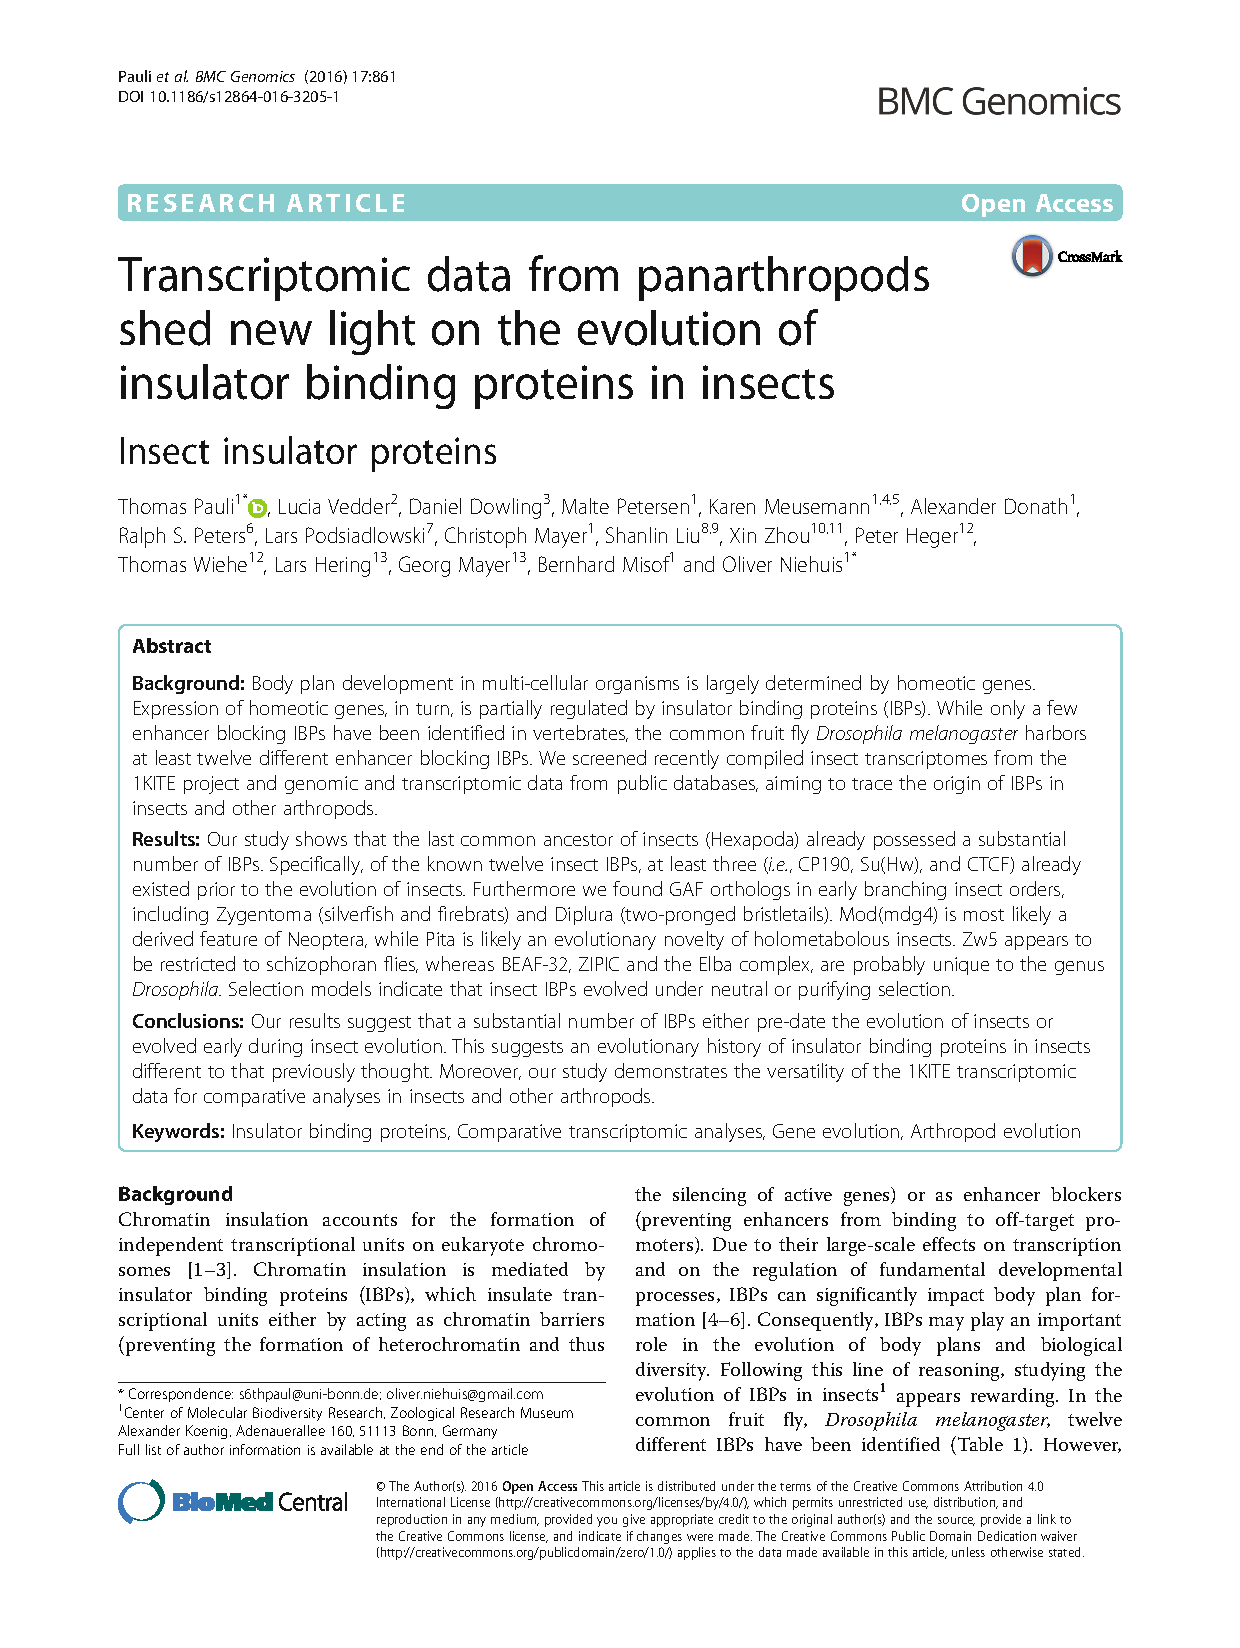
\includepdf[addtotoc={1,section,1,New insights on the evolution of
insulator binding proteins in insects \citep{Pauli2016},app:Pauli2016},pages=-]{appendix/A/Pauli2016}

\includepdf[addtotoc={1,section,1,BaitFisher: A software package for
multispecies target DNA enrichment probe design \citep{Mayer2016},app:Mayer2016},pages=-]{appendix/A/Mayer2016}

